\documentclass[11pt]{beamer}
\usetheme{Boadilla}
\usepackage[utf8]{inputenc}
\usepackage[francais]{babel}
\usepackage[T1]{fontenc}
\usepackage{amsmath}
\usepackage{amsfonts}
\usepackage{amssymb}
\usepackage{graphicx}
\usepackage{tikz}

\def\CS{\text{CS}}
\def\gcup{\displaystyle\cup}
\def\gint{\displaystyle\int}
\def\gsum{\displaystyle\sum\limits}
\def\dxi{\tilde{\delta}^H_{\xi}}
\def\deta{\tilde{\delta}^H_{\eta}}
\def\fxi{\tilde{\mathcal{F}}_{\xi}}
\def\feta{\tilde{\mathcal{F}}_{\eta}}
\def\Vect{\text{Vect}}

\author[M. Brachet]{Matthieu Brachet}
\title[]{Schémas compacts hermitiens sur la Sphère - Applications en climatologie et océanographie numérique}
\date[3-7-2018]{Mardi 3 Juillet 2018} 

\begin{document}

\begin{frame}
\titlepage
\begin{flushright}
\includegraphics[scale=.21]{ul.png}
\includegraphics[scale=.25]{iecl.jpg}
\end{flushright}
\end{frame}

%% ***************************************************************

\begin{frame}
\tableofcontents
\end{frame}

%% ***************************************************************
\section{Contexte}
\begin{frame}{Contexte scientifique général}
\begin{block}{}
Équations aux dérivées partielles d'évolution en géométrie sphérique.
\end{block}
\vspace{.7cm}
\begin{block}{}
Méthodes numériques de haute précision sur grille.
\end{block}
\vspace{.7cm}
\begin{block}{}
Renouvellement des codes de calcul dans le contexte GCM (General Circulation Model).
\end{block}
\end{frame}



\begin{frame}{Problématiques}
\begin{block}{}
Comment généraliser les schémas compacts en géométrie sphérique?
\end{block}
\vspace{.7cm}
\begin{block}{}
Les schémas centrés sur grille sphérique peuvent-ils être utiles pour la propagation en climatologie numérique?
\end{block}
\vspace{.7cm}
\begin{block}{}
Peut-on développer un code démonstrateur Matlab à ce propos?
\end{block}
\end{frame}







%% ***************************************************************
\begin{frame}{}
\begin{block}{Système d'équations Shallow Water sphérique (Eq. de Saint-Venant)}
\begin{equation*}
\text{(SWE) : }\left\lbrace
\begin{array}{rcl}
\dfrac{\partial h^{\star}}{\partial t} + \nabla_T \cdot \left( h^{\star} \mathbf{u} \right) & = & 0\\
\dfrac{\partial \mathbf{u}}{\partial t} + \nabla_T \left( gh + \dfrac{1}{2} |\mathbf{u}|^2 \right) + \left( \zeta + f \right) \mathbf{n} \wedge \mathbf{u} & = & 0.
\end{array}
\right.
\end{equation*}
sur $\mathbb{S}_a^2$ pour $t>0$.
\begin{itemize}
\item $h(t,\mathbf{x})$ : hauteur,
\item $\mathbf{u}(t,\mathbf{x}) \in \mathbb{R}^3$ : vitesse.
\end{itemize}

$g$ : gravité, $f$ : Force de Coriolis, $\zeta = (\nabla_T \wedge \mathbf{u}) \cdot \mathbf{n}$ : vorticité relative, $\mathbf{n}$ : normale extérieure, $h^{\star} = h - h_s$ où $h_s$ est la topographie.
\end{block}

\begin{itemize}
\item Se déduit des équations de Navier-Stokes 3D dans une couche de fluide faible épaisseur.
\end{itemize}
\end{frame}





\begin{frame}{}
\begin{block}{Système d'équations SW linéarisé plan périodique}
\begin{equation*}
\text{(LSWE) : }\left\lbrace
\begin{array}{rcl}
\dfrac{\partial \eta}{\partial t} + H \nabla \cdot \mathbf{v} & = & 0\\
\dfrac{\partial \mathbf{v}}{\partial t} + g \nabla \eta + f \mathbf{n} \wedge \mathbf{v} & = & 0.
\end{array}
\right.
\end{equation*}
sur $[0,L]^2$ et avec $t>0$.

\begin{itemize}
\item $\eta(t,\mathbf{x})$ : perturbation de la hauteur,
\item $\mathbf{v}(t,\mathbf{x})$ : perturbation de la vitesse.
\end{itemize}

$g$ : gravité, $f$ : Force de Coriolis constante, $H$ hauteur constante.
\end{block}

\begin{itemize}
\item Solution analytique disponible en série de Fourier.
\item Permet de tester stabilité et précision d'un schéma.
\end{itemize}
\end{frame}


%% ****************************************************************

\section{}
\begin{frame}{Exemples de grilles sphériques}
\begin{columns}
\column{0.2\textwidth}
\begin{figure}[htbp]
\begin{center}
\includegraphics[height=2.2cm]{lonlat.png}\\
\includegraphics[height=2.35cm]{ico.png}\\
\includegraphics[height=2.25cm]{yinyang.png}\\
\end{center}
\end{figure}

\column{0.7\textwidth}
\begin{itemize}
\item \textbf{Grille longitude-latitude : }
\begin{tiny}
\begin{itemize}
\item Méthodes spectrales : P. N. Swarztrauber 1979;
\item Méthodes Pseudo-spectrales : W. F. Spotz 1998.
\end{itemize} 
\end{tiny}
\vspace{.4cm}

\item \textbf{Grille icosaèdrale : }
\begin{tiny}
\begin{itemize}
\item Volumes Finis (FV) : Dynamico, T. Dubos \textit{et al.} 2014;
\item Galerkin Discontinu (DG) : X. Giraldo \textit{et al.} 2002.
\end{itemize}
\end{tiny}
\vspace{.4cm}

\item \textbf{Grille Yin-Yang : } 
\begin{tiny}
\begin{itemize}
\item FV : X. Li \textit{et al.} 2008;
\item DG : D. M. Hall \textit{et al.} 2003.
\end{itemize}
\end{tiny}
\end{itemize}
\vspace{.2cm}

\pause
Ici : \textbf{Grille Cubed-Sphere}.

\end{columns}
\end{frame}













































%% ***************************************************************

\section{La grille Cubed-Sphere}
\begin{frame}{La Cubed-Sphere}
\begin{columns}
\column{0.4\textwidth}
\begin{figure}[htbp]
\begin{center}
\includegraphics[height=4cm]{cs.png}\\

\end{center}
\end{figure}

\column{0.5\textwidth}
\begin{itemize}
\item Maillage introduit par R. Sadourny (1972).
\vspace{5mm}

\item Possède la topologie du maillage cartésien des 6 faces d'un cube.
\vspace{5mm}

\item Raccord non régulier le long des lignes rouges.
\end{itemize}

\end{columns}
\end{frame}
















\begin{frame}{Construction de la Cubed-Sphere}
\begin{block}{}
\begin{columns}
\column{0.49\textwidth}
Grands cercles sur la Sphere :
\column{0.45\textwidth}
\begin{itemize}
\item $C_{(II)}^1$ et $C_{(II)}^2$ : Est-Ouest,
\item $C_{(V)}^1$ et $C_{(V)}^2$ : Nord-Sud.
\end{itemize}
\end{columns}
\end{block}

\begin{columns}
\column{0.45\textwidth}
\begin{figure}[htbp]
\begin{center}
\includegraphics[scale=0.2]{panelI.jpg}
\end{center}
\end{figure}
\column{0.45\textwidth}
\begin{itemize}
\item $C_{II}^1 = \Vect(\mathbf{i}+\mathbf{k}, \mathbf{j}) \cap \mathbb{S}_a^2$,
\item $C_{II}^2 = R_{\pi/2, (Oy)} ( C_{II}^1 )$ ,
\item $C_V^1 = \Vect(\mathbf{i}-\mathbf{j}, \mathbf{k}) \cap \mathbb{S}_a^2$,
\item $C_V^2 = R_{\pi/2, (Oz)} (C_{V}^1 )$.
\end{itemize}
\begin{block}{}
Les grands cercles $C_{II}^1$, $C_{II}^2$, $C_V^1$ et $C_V^2$ délimitent un \textbf{panel}.
\end{block}
\end{columns}
\end{frame}









\begin{frame}{Construction des points de la Cubed-Sphere}
\begin{columns}
\column{0.4\textwidth}
\begin{figure}[htbp]
\begin{center}
\includegraphics[scale=.27]{cs_cercles.png}
\end{center}
\end{figure}  
\column{0.55\textwidth}
\begin{itemize}
\item 2 ensembles de grands cercles équirépartis $C_i^{(1)}$ et $C_j^{(2)}$, $-N/2 \leq i,j \leq N/2$,

\item $\mathbf{x}_{i,j}=C_i^{(1)} \cap C_j^{(2)}$ forment les points d'un panel de la Cubed-Sphere.

\item $C_0^{(1)}$ et $C_0^{(2)}$ s'intersectent avec un angle de $\pi/2$.
\end{itemize}

\begin{block}{}
On reproduit 6 fois le processus pour recouvrir la sphère $\mathbb{S}_a^2$.
\end{block}

\end{columns}
\end{frame}













\begin{frame}{La grille Cubed-Sphere: 6 panels}
\begin{columns}
\column{0.35\textwidth}
\begin{figure}
\begin{center}
\includegraphics[scale=0.23]{plot_cs2.png}
\caption{Cubed-Sphere de paramètre $N=16$ ($1538$ points de grille).}
\end{center}
\end{figure}
\column{0.65\textwidth}
On définit la grille Cubed-Sphere par
$$
\CS_N = \bigcup_{(k)=(I)}^{(VI)} \left\lbrace \mathbf{x}_{i,j}^{(k)} \text{ t.q. } -N/2 \leq i,j \leq N/2 \right\rbrace
$$
\begin{itemize}
\item $N$ : paramètre de la Cubed-Sphere,
\vspace{.4cm}
\item $6N^2+2$ points sur la Cubed-Sphere.
\vspace{.7cm}
\end{itemize}
\end{columns}
\end{frame}










\begin{frame}{Carte locale sur un panel}
\begin{columns}
\column{0.45\textwidth}
\begin{figure}[htbp]
\begin{center}
\includegraphics[scale=.27]{cs_angles.png}
\end{center}
\caption{Coordonnées locales sur un panel.}
\end{figure}
\column{0.5\textwidth}
\begin{itemize}
\item $(\xi, \eta)$ système d'angles équatoriaux sur chaque panel.
\item $\mathbf{x}$ est repéré par son abscisse $\xi$ et son ordonnée $\eta$.
\item Pour $\mathbf{x}_{i,j}^{(k)} \in \CS_N$, on a $(\xi_i, \eta_j) = (i \Delta \xi, j \Delta \eta)$ avec 
$$
\Delta \xi = \Delta \eta = \dfrac{\pi}{2N}.
$$
\end{itemize}
\end{columns}
\end{frame}











\begin{frame}{Bases locales sur un panel}
\begin{columns}
\column{0.45\textwidth}
\begin{figure}[htbp]
\begin{center}
\includegraphics[scale=.27]{cs_angles.png}
\end{center}
\end{figure}
\column{0.5\textwidth}
\begin{itemize}
\item La base de référence en $\mathbf{x}$ est $$(\mathbf{g}_{\xi}, \mathbf{g}_{\eta}) = (\partial_{\xi} \mathbf{x}, \partial_{\eta} \mathbf{x}).$$
\item Le tenseur métrique en $\mathbf{x} \in \mathbb{S}_a^2$ est
\begin{equation*}
G=\begin{bmatrix}
\mathbf{g}_{\xi} \cdot \mathbf{g}_{\xi} & \mathbf{g}_{\xi} \cdot \mathbf{g}_{\eta} \\
\mathbf{g}_{\eta} \cdot \mathbf{g}_{\xi} & \mathbf{g}_{\eta} \cdot \mathbf{g}_{\eta} 
\end{bmatrix}
\end{equation*}
\item La base duale en $\mathbf{x} \in \mathbb{S}^2_a $ est $(\mathbf{g}^\xi,\mathbf{g}^\eta)$ donnée par
$$
\begin{bmatrix}
\mathbf{g}^{\xi} \\ \mathbf{g}^{\eta} 
\end{bmatrix}
=
\mathbf{G}^{-1} \cdot
\begin{bmatrix}
\mathbf{g}_{\xi} \\ \mathbf{g}_{\eta} 
\end{bmatrix}.
$$
\end{itemize}
\end{columns}
\end{frame}

























\begin{frame}{Produit scalaire discret sur la Cubed-Sphere}
\begin{block}{}
Une \textbf{fonction de grille} est définie aux points de la grille :
$$\mathfrak{u} : \mathbf{x}_{i,j}^{(k)} \in \CS_N \mapsto \mathfrak{u}_{i,j}^{(k)}.$$
Soit $u : \mathbb{S}_a^2 \mapsto \mathbb{C}$, alors $$u^* = u_{| \CS_N}. $$
\end{block}
\begin{block}{Produit scalaire discret sur la Cubed-Sphere}
Analogue discret de $<u,v> = \gint_{\mathbb{S}_a^2} u(\mathbf{x}) \bar{v}(\mathbf{x}) d \sigma(\mathbf{x})$ :
$$<\mathfrak{u},\mathfrak{v}>_{\CS_N} = \gsum_{(k) = (I)}^{(VI)} \gsum_{-N/2 \leq i,j \leq N/2} \omega_{i,j} \sqrt{\bar{\mathbf{G}}_{i,j}} \mathfrak{u}_{i,j}^{(k)} \bar{\mathfrak{v}}_{i,j}^{(k)}$$
avec les coefficients $\omega_{i,j}$ positifs et $\bar{\mathbf{G}}_{i,j} = \det ( \mathbf{G}(\mathbf{x}_{i,j}^{(k)}))$.
\end{block}
\end{frame}














\begin{frame}{Bilan pour la Cubed-Sphere}
\begin{block}{Maillage Cubed-Sphere}
\begin{itemize}
\item Structure basée sur des grands cercles.
\item Géométrie par panel quasi-cartésienne.
\item Pas de discrétisation régulier par panel avec
$$
\Delta \xi  = \Delta \eta = \dfrac{\pi}{2N}
$$
\item Produit scalaire discret défini de façon naturelle.
\end{itemize}
\end{block}
\end{frame}















%% ***************************************************************
\section{Opérateurs discrets sur la Cubed-Sphere}
\begin{frame}{Opérateurs différentiels sur la Cubed-Sphere}
\begin{exampleblock}{}
Les opérateurs gradient, divergence et rotationnel sont définis sur la sphère de façon intrinsèque.
\end{exampleblock}
\begin{block}{Expression en coordonnées $(\xi, \eta)$}
\begin{itemize}
\item \textbf{Gradient :}
$$
\nabla_T h = \mathbf{g}^{\xi} \dfrac{\partial h}{\partial \xi} + \mathbf{g}^{\eta} \dfrac{\partial h}{\partial \eta},
$$
\item \textbf{Divergence :}
$$
\nabla_T \cdot \mathbf{u} = \mathbf{g}^{\xi} \cdot \dfrac{\partial \mathbf{u}}{\partial \xi} + \mathbf{g}^{\eta} \cdot \dfrac{\partial \mathbf{u}}{\partial \eta},
$$
\item \textbf{Vorticité :}
$$
\text{vort}(\mathbf{u}) = \left( \mathbf{g}^{\xi} \wedge \dfrac{\partial \mathbf{u}}{\partial \xi} + \mathbf{g}^{\eta} \wedge \dfrac{\partial \mathbf{u}}{\partial \eta} \right) \cdot \dfrac{\mathbf{x}}{a}.
$$
\end{itemize}
\end{block}
\end{frame}
















\begin{frame}{Approximation de $\partial_{\xi}$}
\begin{columns}
\column{0.5\textwidth}
$u_{i,j}^{(k)}$ donné en tout point de $\CS_N$.
\begin{figure}
\begin{center}
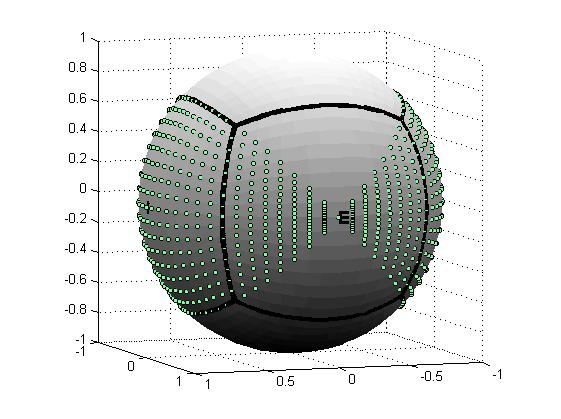
\includegraphics[scale=.3]{fig22.jpg}
\end{center}
\end{figure}
\column{0.5\textwidth}
\begin{block}{Objectif}
Approcher $\dfrac{\partial}{\partial \xi}$ avec la meilleure précision possible.
\end{block}
\begin{block}{}
\begin{itemize}
\item Assigner les données en tout point de chaque cercle vert.
\item Définir une approximation de $\dfrac{\partial}{\partial \xi}$ appliquée à ces données.
\item Répéter sur 6 réseaux de grands cercles associés à la Cubed-Sphere.
\end{itemize}
\end{block}
\end{columns}
\end{frame}













\section{Schéma compact pour les équations de propagation sur la sphère}
\begin{frame}{Discrétisation sur un grand cercle}
On se donne $(\mathfrak{u}_j)_{j\in \mathbb{Z}}$ une fonction de grille périodique
\begin{figure}[htbp]
\begin{center}
\begin{tikzpicture}[scale=1]
	\draw [>=stealth, <->] (-2,0.2) -- (-1,.2) ;
	\draw (-1.5,.3) node[above] {$\Delta \xi$} ;
	\draw [>=stealth, <->] (-3,0) -- (3,0) ;
	\draw (-2,0) node {$\bullet$} ;
	\draw (-2,-.2) node[below] {$\cdots$} ;
	\draw (-1,0) node {$\bullet$} ;
	\draw (-1,-.2) node[below] {$\mathfrak{u}_{j-1}$} ;
	\draw (0,0) node {$\bullet$} ;
	\draw (0,-.2) node[below] {$\mathfrak{u}_j$} ;
	\draw (1,0) node {$\bullet$} ;
	\draw (1,-.2) node[below] {$\mathfrak{u}_{j+1}$} ;
	\draw (2,0) node {$\bullet$} ;
	\draw (2,-.2) node[below] {$\cdots$} ;
\end{tikzpicture}
\end{center}
\end{figure}

\begin{block}{Formule locale d'ordre 2 :}
\begin{itemize}
\item L'opérateur $\delta_{\xi}$ est défini par
$$
\dfrac{\mathfrak{u}_{j+1}-\mathfrak{u}_{j-1}}{2 \Delta \xi} = \delta_{\xi} \mathfrak{u}_j \text{ avec } j \in \mathbb{Z},
$$
\item Précis au 2-nd ordre :
$$
\delta_{\xi} u^*_j = \partial_{\xi} u_j + \mathcal{O} \left( \Delta \xi^2 \right)
$$
avec $u \in \mathcal{C}^3$.
\end{itemize}
\end{block}
\end{frame}






\begin{frame}{}
\begin{block}{Opérateur hermitien $\delta_{\xi}^H$ :}
L'opérateur de \textbf{dérivation hermitien} est défini par
$$
\delta_{\xi}^H = \sigma_{\xi}^{-1} \circ \delta_{\xi}
$$
où $\sigma_{\xi}$ et $\delta_{\xi}$ sont définis par
$$
\sigma_{\xi} \mathfrak{u}_{\xi,j} = \dfrac{1}{6}\mathfrak{u}_{\xi,j-1} + \dfrac{4}{6}\mathfrak{u}_{\xi,j} + \dfrac{1}{6} \mathfrak{u}_{\xi,j+1} \text{ et } \delta_{\xi} \mathfrak{u}_j= \dfrac{\mathfrak{u}_{j+1}-\mathfrak{u}_{j-1}}{2 \Delta \xi}.
$$
\end{block}
\begin{block}{Approximation d'ordre 4 :}
Approximation de la dérivée première à l'ordre 4:
$$
\delta_{\xi}^H u^*_j = \partial_{\xi} u_j + \mathcal{O} \left( \Delta \xi^4 \right)
$$
avec $u \in \mathcal{C}^5$.
\end{block}
\end{frame}










\begin{frame}{Opérateur $\dxi$}
\begin{columns}
\column{0.45\textwidth}
\textbf{Procédure pour $\dxi$ :}
\begin{enumerate}
\item Transfert des données sur les panels (I) et (III).
\item Complétion des données sur les panels (II) et (IV) par \textbf{spline cubique},
\item Calcul de la dérivée approchée en utilisant $\delta_{\xi}^H$.
\end{enumerate}
\column{0.5\textwidth}
\begin{center}
\includegraphics[scale=.28]{CS_interp.png}
\end{center}
\end{columns}
$\Rightarrow$ \textbf{Approximation :} remplacer systématiquement $\dfrac{\partial}{\partial \xi}$ par $\dxi$.
\end{frame}


















\begin{frame}{Opérateurs différentiels discrets sur la Cubed-Sphere}
Les opérateurs différentiels discrets sont définis pour toutes fonctions de grilles $\mathfrak{h}$ et $\mathfrak{u}$ par
\begin{block}{}
\begin{itemize}
\item \textbf{Gradient discret:}
$$
\nabla_{T,\Delta} \mathfrak{h} = \mathbf{g}^{\xi} \dxi \mathfrak{h} + \mathbf{g}^{\eta} \deta \mathfrak{h},
$$
\item \textbf{Divergence discrète :}
$$
\nabla_{T,\Delta} \cdot \mathfrak{u} = \mathbf{g}^{\xi} \cdot \dxi \mathfrak{u} + \mathbf{g}^{\eta} \cdot \deta \mathfrak{u},
$$
\item \textbf{Vorticité discrète :}
$$
\text{vort}_{\Delta} (\mathfrak{u}) = \left( \mathbf{g}^{\xi} \wedge \dxi \mathfrak{u} + \mathbf{g}^{\eta} \wedge \deta \mathfrak{u} \right) \cdot \dfrac{\mathbf{x}}{a}.
$$
\end{itemize}
avec $\Delta \xi = \Delta \eta = \dfrac{\pi}{2N}$.
\end{block}
\end{frame}
















\begin{frame}{Consistance des opérateurs discrets}
Soit $h$ une fonction scalaire et $\mathbf{u}$ un champ vectoriel sur $\mathbb{S}_a^2$. Pour $h$ et $\mathbf{u}$ réguliers on a :
\begin{block}{}
\begin{itemize}
\item \textbf{Consistance du gradient :}
$$
(\nabla_T h)^* - \nabla_{T,\Delta} h^* = \mathcal{O}(\Delta \xi^3),
$$
\item \textbf{Consistance de la divergence :}
$$
(\nabla_T \cdot \mathbf{u})^* - \nabla_{T,\Delta} \cdot \mathbf{u}^* = \mathcal{O}(\Delta \xi^3),
$$
\item \textbf{Consistance de la vorticité :}
$$
\text{vort}(\mathbf{u})^* - \text{vort}_{\Delta}(\mathbf{u}^*) = \mathcal{O}(\Delta \xi^3).
$$
\end{itemize}
\end{block}
\begin{alertblock}{}
\textbf{Ordre 4} observé dans les expériences numériques.
\end{alertblock}
\end{frame}


























\begin{frame}{Bilan sur les opérateurs discrets}
\begin{block}{}
\begin{itemize}
\item Procédure de construction systématique d'opérateurs discrets centrés.
\vspace{.4cm}
\item Remplacement possible de $\delta_{\xi}^H$ par tout autre opérateur aux différences.
\vspace{.4cm}
\item Approximation par spline cubique limite la montée en ordre.
\end{itemize}
\end{block}
\end{frame}










%% *****************************************************************
\begin{frame}{Equation de transport 1D}
On considère l'équation :
$$
\left\lbrace
\begin{array}{rcl}
\dfrac{\partial u}{\partial t} + c \dfrac{\partial u}{\partial x} & = & 0 \\
u(t=0,x) & = & u_0(x)
\end{array}
\right. \text{ pour } x \in [0,L] \text{ et } t>0.
$$
\begin{block}{}
\textbf{Première étape : discrétisation en espace.}
\end{block}
Equation semi-discrétisée, on cherche $t \mapsto \mathfrak{u}(t)$ solution de :
$$
\left\lbrace
\begin{array}{rcl}
\dfrac{\partial \mathfrak{u}}{\partial t} + c \delta_x^H \mathfrak{u} & = & 0 \\
\mathfrak{u}(t=0) & = & u_0^*
\end{array}
\right. \text{ pour } x \in [0,L] \text{ et } t>0,
$$
On a $\mathfrak{u} = (\mathfrak{u}_0, \cdots , \mathfrak{u}_{N-1})$, alors $\mathfrak{u}_j(t) \approx u(t, x_j)$.
\end{frame}













\begin{frame}{}
\begin{block}{Proposition}
Pour $u$ est régulière, alors on a
$$
\| \mathfrak{u}(t) - u(t,\cdot)^* \|_{h,\text{pér}} \leq C t \Delta \xi^4 \| \partial_{\xi}^{(5)}u \|_{\infty}
$$
avec $C>0$ indépendant de $t$, $\Delta \xi$ et $u$.
\end{block}
\end{frame}













\begin{frame}{Discrétisation en temps}
\begin{block}{Runge-Kutta d'ordre 4 + Filtre spatial}
\begin{enumerate}
\item $K^{(1)} = - c \delta_{\xi}^H \mathfrak{u}^n$,
\item $K^{(2)} = - c \delta_{\xi}^H \left( \mathfrak{u}^n + \dfrac{\Delta t}{2} K^{(1)} \right)$,
\item $K^{(3)} = - c \delta_{\xi}^H \left( \mathfrak{u}^n + \dfrac{\Delta t}{2} K^{(2)} \right)$,
\item $K^{(4)} = - c \delta_{\xi}^H \left( \mathfrak{u}^n + \Delta t K^{(3)} \right)$
\item $\hat{\mathfrak{u}}^{n+1} = \mathfrak{u}^n + \frac{\Delta t}{6} \left( K^{(1)} + 2 K^{(2)} + 2 K^{(3)} + K^{(4)} \right)$
\item $\mathfrak{u}^{n+1} = \mathcal{F}(\hat{\mathfrak{u}}^{n+1})$
\end{enumerate}
\end{block}

\begin{block}{}
Deux sources de dissipation : RK4 et $\mathcal{F}$.
\end{block}

\end{frame}





















\begin{frame}{Opérateur de filtrage}
L'opérateur de filtrage est donné par
$$
\mathcal{F} (\mathfrak{u})_j = \gsum_{p=-5}^5 f_p \mathfrak{u}_{p+j} 
$$
\begin{columns}
\column{0.45\textwidth}
Les coefficients sont donnés par
$$
\begin{bmatrix}
f_0\\
f_1 = f_{-1}\\
f_2 = f_{-2}\\
f_3 = f_{-3}\\
f_4 = f_{-4}\\
f_5 = f_{-5}\\
\end{bmatrix} =
\begin{bmatrix}
772/1024\\
420/1024\\
-240/1024\\
90/1024\\
-20/1024\\
2/1024\\
\end{bmatrix}
$$
\column{0.45\textwidth}
\begin{block}{}
Si $u \in \mathcal{C}^{10}$, on a :
$$
\mathcal{F}(\mathfrak{u}^*)_j = u(x_j) + \mathcal{O} \left( \Delta \xi^{10} \right).
$$
\end{block}
\begin{block}{}
\begin{itemize}
\item $\mathcal{F}$ annule complètement le mode $\pm1$ : $\mathcal{F}(\pm1)=0$,
\item amméliore la dispersion
\item \href{run:./simus/creneau_cfl1.avi}{Créneau sans filtre},
\item \href{run:./simus/creneau_ftr10_cfl1.avi}{Créneau avec filtre},
\end{itemize}
\end{block}
\end{columns}
\end{frame}











\begin{frame}{}
\begin{block}{Proposition}
Le schéma est conservatif au sens où
$$
<\mathfrak{u}^{n+1},\mathfrak{1}>_{\text{pér}} = <\mathfrak{u}^{n},\mathfrak{1}>_{\text{pér}}
$$
pour tout $n \in \mathbb{N}$.
\end{block}
\begin{block}{Proposition}
Le schéma est stable sous la condition
$$
\dfrac{c \Delta t}{\Delta \xi} \leq \lambda_{10}.
$$
\begin{itemize}
\item Estimation numérique $\lambda_{10} > 1.68$.
\end{itemize} 
\end{block}
\end{frame}















\begin{frame}{Equation LSWE semi-discrétisée}
\begin{columns}
\column{0.45\textwidth}
Domaine considéré : $[0,1]^2$.

\textbf{Equation semi-discrétisée :}
$$
\left\lbrace
\begin{array}{rcl}
\dfrac{d \eta}{d t} + H \left( \delta_x^H \mathfrak{u} + \delta_y^H \mathfrak{v} \right) & = & 0 \\
\dfrac{d \mathfrak{u}}{d t} + g \delta_x^H \eta - f\mathfrak{v} & = & 0\\
\dfrac{d \mathfrak{v}}{d t} + g \delta_y^H \eta + f\mathfrak{u} & = & 0
\end{array}
\right.
$$
Résolution en temps par RK4 avec étape de filtrage.
\begin{block}{Proposition :}
Le schéma est d'ordre 4 en espace et en temps.
\end{block}
\column{0.45\textwidth}
\begin{block}{Proposition :}
le schéma est conservatif au sens :
$$
<\eta^{n+1},\mathfrak{1}>_{\text{pér}} = <\eta^{n},\mathfrak{1}>_{\text{pér}}
$$
pour tout $n \in \mathbb{N}$.
\end{block}
\begin{block}{Proposition :}
Le schéma est stable sous la condition CFL
$$
\Delta t \leq \dfrac{2 \sqrt{2}}{\sqrt{\dfrac{6gH}{\Delta \xi^2} + f^2}}.
$$
\end{block}
\end{columns}
\end{frame}





































%% *****************************************************************
\section{Résultats numériques sur la sphère}
\begin{frame}{Méthode des lignes}
On considère le problème pour $q : (t,\mathbf{x}) \mapsto q(t,\mathbf{x})$
$$
\left\lbrace
\begin{array}{rcl}
\dfrac{\partial q}{\partial t} & = & F(q,t) \\
q(t=0,\mathbf{x}) & = & q_0(\mathbf{x})
\end{array}
\right. \text{ avec } \mathbf{x} \in \mathbb{S}_a^2.
$$
\begin{block}{}
\textbf{Première étape : } discrétisation en espace centrée.
\end{block}
$$
\left\lbrace
\begin{array}{rcl}
\dfrac{d \mathfrak{q}}{d t} & = & F_{\Delta}(\mathfrak{q},t) \\
\mathfrak{q}(t=0) & = & q_0^*
\end{array}
\right. \text{ avec } \mathbf{x} \in \mathbb{S}_a^2.
$$
\begin{block}{}
\textbf{Seconde étape : } discrétisation en temps : RK4 avec étape de filtrage.
\end{block}
\end{frame}






\begin{frame}{Schéma de référence}
\begin{block}{Runge-Kutta d'ordre 4 + Filtre spatial
}
\begin{enumerate}
\item $K_1 = F_{\Delta}(\mathfrak{q}^n, t^n)$,
\item $K_2 = F_{\Delta}(\mathfrak{q}^n + \frac{\Delta t}{2} K_1, t^n + \frac{\Delta t}{2})$,
\item $K_3 = F_{\Delta}(\mathfrak{q}^n + \frac{\Delta t}{2} K_2, t^n + \frac{\Delta t}{2})$,
\item $K_4 = F_{\Delta}(\mathfrak{q}^n + \Delta t K_3, t^n + \Delta t)$
\item $\hat{\mathfrak{q}}^{n+1} = \mathfrak{q}^n + \frac{\Delta t}{6} \left( K_1 + 2 K_2 + 2 K_3 + K_4 \right)$
\item $\mathfrak{q}^{n+1} = \mathcal{F}(\hat{\mathfrak{q}}^{n+1})$
\end{enumerate}
\end{block}
\end{frame}










\begin{frame}{Opérateur de filtrage sur la sphère}
En suivant le même procédé que pour $\dxi$, on construit les opérateurs de filtrage $\fxi$ et $\feta$. On définit alors :
$$
\mathcal{F} = \dfrac{1}{2} \left( \fxi \circ \feta + \feta \circ \fxi \right),
$$
\begin{block}{}
Si $h$ est une fonction régulière sur la sphère, on a:
$$
\mathcal{F}(h^*) - h^* = \mathcal{O} \left( \Delta \xi^4 \right).
$$
\end{block}
\end{frame}











\begin{frame}{Cas test en climatologie numérique}
\begin{itemize}
\item Test de transport solide :
\begin{itemize}
\item Cosine Bell (Test 1 de Williamson \textit{et al.} (1992)),
\end{itemize}
\item Transport de scalaires passifs :
\begin{itemize}
\item R. Nair et P. Lauritzen (2010),
\end{itemize}
\item Tests déformationnels :
\begin{itemize}
\item Test de R. Nair et B. Machenhauer (2002),
\item Test de R. Nair et C. Jablonowski (2008),
\end{itemize}
\item Tests pour les équations SWE :
\begin{itemize}
\item "Montagne isolée" (test 5 de  Williamson \textit{et al.}),
\item Ondes de Rossby-Haurwitz (test 6 de  Williamson \textit{et al.}),
\item Test de J. Galewsky : instabilité barotropique (2004),
\end{itemize}
\item Tests pour LSWE sphérique :
\begin{itemize}
\item Ondes sphériques, O. Shamir et N. Paldor (2016).
\end{itemize}
\end{itemize}
\end{frame}





















\begin{frame}{Test de R. Nair et C. Jablonowski (2008)}
On considère l'équation
$$
\left\lbrace
\begin{array}{rcl}
\dfrac{\partial h}{\partial t} + c(t,\mathbf{x}) \cdot \nabla_T h & = & 0  \\
h(t=0,\mathbf{x}) & = & h_0(\mathbf{x})
\end{array}
\right. \text{ avec } \mathbf{x} \in \mathbb{S}_a^2.
$$
où $h$ est une densité de polluant.
\begin{exampleblock}{Test de R. Nair et C. Jablonowski (2008)}
\begin{itemize}
\item Déplacement d'un vortex autour de la sphère,
\item Une solution analytique est disponible $\Rightarrow$ mesure de l'erreur relative.
\end{itemize}
\end{exampleblock}
\end{frame}



\begin{frame}{}
\begin{figure}
\begin{center}
\href{run:./simus/ref_7363145849_test_2.avi}{\includegraphics[height=5cm]{NJ_init.png}}
\end{center}
\caption{Condition initiale sur une grille $6 \times 32 \times 32$ (CFL=0.7).}
\end{figure}
\end{frame}







\begin{frame}
\begin{figure}
\begin{center}
\includegraphics[height=5cm]{rate_NJ1.png}
\end{center}
\caption{Erreur relative pour l'équation d'advection linéaire (CFL=0.7). Ordre observé entre $3.5$ et $4$.}
\end{figure}
\end{frame}

















\begin{frame}{Equation d'advection non linéaire}

On considère l'équation
$$
\left\lbrace
\begin{array}{rcl}
\dfrac{\partial h}{\partial t} + \nabla_T \cdot F(h, \mathbf{x}) & = & 0  \\
h(t=0,\mathbf{x}) & = & h_0(\mathbf{x})
\end{array}
\right. \text{ avec } \mathbf{x} \in \mathbb{S}_1^2.
$$

avec $F(h, \mathbf{x}) = \dfrac{1}{2} h^2 \mathbf{n} \wedge (\mathbf{i} + \mathbf{j} + \mathbf{k})$ 

\begin{exampleblock}{Test de M. Ben-Artzi \text{et al.} (2013)}
\begin{itemize}
\item Conservation de la solution stationnaire 
$$
h_0(x,y,z) = \dfrac{x+y+z}{\sqrt{3}}.
$$
\item La masse doit être conservée.
\end{itemize}
\end{exampleblock}
\end{frame}



\begin{frame}
\begin{figure}[htbp]
\begin{center}
\includegraphics[height=5cm]{rateBA_test3.png}
\end{center}
\caption{Erreur et taux de convergence pour le test stationnaire de l'équation d'advection non linéaire en fonction de $\Delta = a \Delta \xi$. Le pas de temps est donné par $\Delta t = 0.96 \Delta \xi / \pi$. Le temps final est $t=6$.}
\label{fig:benartzi_test3}
\end{figure}
\end{frame}





\begin{frame}
\begin{figure}[htbp]
\begin{center}
\includegraphics[height=4cm]{erreur_test3.png}
\includegraphics[height=4cm]{cons_test3.png}
\end{center}
\caption{ L'erreur relative en norme et l'erreur de conservation pour l'équation d'advection non linéaire. On a $\Delta t = 0.96 \Delta \xi / \pi$. Le temps final est $t=6$. Le paramètre de la Cubed-Sphere est $N=32$.}
\label{fig:benartzi_test3_hist}
\end{figure}
\end{frame}














%% ****************************************************************************************************************************************

\begin{frame}{Equation SWE sphérique}
\begin{block}{}
\begin{equation}
\text{(SWE) : }\left\lbrace
\begin{array}{rcl}
\dfrac{\partial h^{\star}}{\partial t} + \nabla_T \cdot \left( h^{\star} \mathbf{u} \right) & = & 0 \\
\dfrac{\partial \mathbf{u}}{\partial t} + \nabla_T \left( \dfrac{1}{2}|\mathbf{u}|^2 + gh \right) + \left( f + \zeta \right) \mathbf{n} \times \mathbf{u} & = & 0
\end{array}
\right.
\end{equation}
où  
\begin{itemize}
\item $h$ est l'épaisseur de fluide et $\mathbf{v}$ le champ de vitesse tangent,
\item $h^{\star}=h-h_s$ avec $h_s$ représentant la topographie, en général on aura $h_s=0$,
\item $\mathbf{n}$ la normale extérieure, 
\item $\zeta = \left( \nabla_T \times \mathbf{u} \right) \cdot \mathbf{n}$ est la vorticité,
\item $f$ est le paramètre de Coriolis.
\end{itemize}
\end{block}
\end{frame}

%% ***************************************************************************************************************************************

\begin{frame}{Propriétés de conservation}
\begin{block}{}
Si $(h, \mathbf{u})$ est solution des équations SWE, les quantités suivantes sont conservées au cours du temps
\begin{itemize}
\item \textbf{masse :} 
$t \mapsto \gint_{\mathbb{S}^2_a} h d \sigma(\mathbf{x})$
\item \textbf{énergie :}
$t \mapsto \gint_{\mathbb{S}^2_a} \left( \dfrac{1}{2}g(h^2 - h_s^2) + \dfrac{1}{2} h | \mathbf{u} |^2 \right) d \sigma(\mathbf{x})$
\item \textbf{enstrophie potentielle :}
$t \mapsto \gint_{\mathbb{S}^2_a} \dfrac{\left( f + \zeta \right)^2}{2gh} d \sigma(\mathbf{x})$
\end{itemize}
\end{block}
\end{frame}

%% ***************************************************************************************************************************************

\begin{frame}{Test 2 de Williamson \textit{et al.}}

\begin{exampleblock}{Solution stationnaire :}
\begin{itemize}
\item $h = h_0 - \dfrac{1}{g} \left( a \Omega u_0 + \dfrac{u_0^2}{2} \right)\left( - \cos \lambda \cos \theta \sin \alpha + \sin \theta \cos \alpha \right)^2$
\item $\mathbf{u} = u \mathbf{e}_{\lambda}+ v \mathbf{e}_{\theta}$ avec :
\begin{equation*}
\left\lbrace \begin{array}{rcl}
 u & = & u_0 ( \cos \theta \cos \alpha + \cos \lambda \sin \theta \sin \alpha)\\
 v & = & -u_0 \sin \lambda \sin \alpha
 \end{array} \right.
\end{equation*}
\end{itemize}
\end{exampleblock}
\end{frame}

%% ***************************************************************************************************************************************

\begin{frame}{}
\begin{figure}
\includegraphics[height=3cm]{ref_7369088270_snapshot_err_color.png}
\includegraphics[height=3cm]{ref_7369088270_snapshot_intermediaire598.png}
\end{figure}
\begin{itemize}
\item Solution stationnaire avec $\alpha=\pi/4$, la taille de grille est $6 \times 32 \times 32$, le temps final est $T=6$ jours.
\item Erreur relative sur $h$ au temps finale (gauche).
\item $h$ au temps final (droite),
\item $\Delta t \approx 10$ minutes.
\item Absence d'oscillations parasites.
\end{itemize}
\end{frame}

%% ***************************************************************************************************************************************

\begin{frame}{Analyse de l'erreur}
\begin{figure}
\includegraphics[height=4cm]{rate_W2_pi4.png}
\end{figure}
\begin{itemize}
\item  On mesure l'erreur relative à $T=6$ jours  :
$$
\dfrac{\| \mathfrak{h}_0 - \mathfrak{h}^n \|}{\| \mathfrak{h}_0 \|}
$$
\item Convergence à l'ordre 4.
\end{itemize}
\end{frame}








\begin{frame}{}
Au temps $t = 5$ jours avec $\alpha = \pi/4$ :
\begin{equation*}
\begin{array}{|c|c|}
\hline
\hline
 & \textbf{Erreur en norme infinie} \\
\hline
 \textbf{Schéma présent :} & 2.75 (-6) \\
 \textbf{VF d'ordre 4 [Chen et al., 2008]} : & 5.86 (-6) \\
 \textbf{VF d'ordre 4 [Ullrich et al., 2011]} : & 1.47 (-6) \\
\hline
\hline
\end{array}
\end{equation*}
pour une grille $6 \times 32 \times 32$ et CFL$=0.9$.
\begin{block}{}
\begin{itemize}
\item Très bonne précision pour ce test.
\item Erreur comprise entre Chen \textit{et al.} et Ullrich \textit{et al.} (VF décentrés).
\end{itemize}
\end{block}
\end{frame}







%% ***************************************************************************************************************************************

\begin{frame}{Conservation}
\begin{figure}
\includegraphics[height=5cm]{ref_7369088270_conservationA.png}
\end{figure}
\begin{itemize}
\item Erreur relative de conservation pour une grille : $6 \times 32 \times 32$ avec $\alpha=\pi/4$ (713 it.).
\item Erreur relative maximale observée sur 6 jours : $7 \times 10^{-9}$.
\end{itemize}
\end{frame}





























%% **************************************************************************************************************************************

\begin{frame}{Test 5 de Williamson \textit{et al.}}

\begin{exampleblock}{}
Test similaire au précédent avec $\alpha = 0$ :

\begin{itemize}
\item $h = h_0 - \dfrac{1}{g} \left( a \Omega u_0 + \dfrac{u_0^2}{2} \right)(\sin \theta)^2$
\item $\mathbf{u} = u_0 \cos \theta \mathbf{e}_{\lambda}$.
\end{itemize}

Cette solution stationnaire est perturbée par une montagne isolée:

$$h_s = h_{s_0} \left( 1 - \dfrac{r}{R} \right)$$

avec $h_{s_0}=2000m$ and $r^2=\min(R^2, (\lambda + \pi/2)^2+(\theta - \pi/6)^2)$, $R=\pi/9$.
\end{exampleblock}
\end{frame}




%% ***************************************************************************************************************************************

\begin{frame}{Conservation}
\begin{figure}
\href{run:./simus/ref_7367913664.mpeg.avi}{\includegraphics[height=4cm]{ref_7368974583_conservationA.jpg}}
\end{figure}
\begin{itemize}
\item La grille est $6 \times 32 \times 32$.
\item Résultats semblables à ceux de DG et VF.
\item La masse et l'énergie sont conservées avec une erreur relative proche de $10^{-5}$.
\item L'enstrophie potentielle est conservée avec une erreur relative proche de $10^{-4}$.
\end{itemize}
\end{frame}





\begin{frame}{}
Au temps $t = 15$ jours, erreurs relatives de conservation :
\begin{equation*}
\begin{array}{|c|c|c|}
\hline
\hline
 & \textbf{Energie} & \textbf{Enst. pot.} \\
\hline
 \textbf{Schéma présent :} & 1.6 (-5) &-0.9 (-4) \\
 \textbf{VF4 [Chen et al., 2008] (N=32)} : & -4 (-6) & -1.1 (-4) \\
 \textbf{VF4 [Ullrich et al., 2011]} (N=40) : & -3 (-4) & -1.1 (-4) \\
\hline
\hline
\end{array}
\end{equation*}
pour une grille $6 \times 32 \times 32$ (grille grossière) et CFL$=0.9$.
\begin{block}{}
Résultats analogues à VF4.
\end{block}
\end{frame}


























% ***************************************************************************************************************

\begin{frame}{Instabilité Barotrope [J. Galewsky \textit{et al.}, 2004]}
\begin{exampleblock}{}
Une solution stationnaire instable est donnée par
\begin{equation}
\begin{array}{rcl}
\bar{h}(\theta) & = & h_0 + \dfrac{1}{g}\gint^{\theta}_{-\pi/2} a u(\tau) \left[ f + \dfrac{\tan(\tau)}{a} u(\tau) \right] d \tau \\
\mathbf{u}(\lambda,\theta) & = & u(\theta) \mathbf{e}_{\lambda}
\end{array}
\end{equation}
avec :
\begin{itemize}
\item le paramètre de Coriolis $f = 2 \Omega \sin \theta$,
\item $u(\theta)=\left\lbrace
\begin{array}{ll}
\dfrac{u_{max}}{e_n} \exp\left( \dfrac{1}{(\theta-\theta_0)(\theta-\theta_1)} \right) & \text{ if } \theta_0 \leq \theta \leq \theta_1 \\
0 & \text{ else}
\end{array}\right.$\\
 avec $e_n=C^{ste}$, $u_{max} = 80 ms^{-1}$, $\theta_0 = \pi/7$ and $\theta_1 = \pi/2 - \theta_0$.
\end{itemize}
\end{exampleblock}
\end{frame}


%% ***************************************************************************************************************************************

\begin{frame}{}
\begin{exampleblock}{Donnée initiale}
La fonction précédente est perturbée avec :
\begin{itemize}
\item vitesse zonale :
$$\mathbf{u}(\lambda,\theta) = u(\theta) \mathbf{e}_{\lambda}$$
\item perturbation de $h$ par $\bar{h}$:
$$h(\lambda,\theta) = \bar{h}(\lambda,\theta) + \hat{h} \cos \theta \exp \left[ - \left( \dfrac{\lambda}{\alpha} \right)^2 - \left( \dfrac{\theta_2 - \theta}{\beta} \right)^2 \right] \text{, } \hat{h}/\bar{h} \approx 1 \%$$
avec $\theta_2 = \pi/4$, $\alpha = 1/3$ and $\beta = 1/15$.
\end{itemize}
\end{exampleblock}
\begin{block}{}
Ce test est difficile pour la Cubed-Sphere :
\begin{itemize}
\item $h$ varie le long du panel (V),
\item la perturbation initiale est localisée entre les panels (I) et (V).
\end{itemize}
\end{block}
\end{frame}

%% ***************************************************************************************************************************************

\begin{frame}{}
\begin{figure}
\href{run:./simus/ref_7372378359.avi}{\includegraphics[height=5cm]{ref_7369437806_snapshot_intermediaire599.jpg}}
\end{figure}
\begin{itemize}
\item On représente la vorticité au temps $t=6$ jours sur une grille $6 \times 128 \times 128$ (grille fine).

\item Comparaisons avec DG et VF d'ordre 4 : nombre de vortex, position, ...

\item Résultats semblables.
\end{itemize}
\end{frame}

%%% ***************************************************************************************************************************************

\begin{frame}{Conservation : masse, énergie et enstrophie potentielle}
\begin{figure}
\includegraphics[height=4cm]{ref_7368306511_massenergy.png}
\includegraphics[height=4cm]{ref_7368306511_enstrophy.png}
\end{figure}
\begin{itemize}
\item Conservation de la masse et de l'énergie (gauche) et de l'enstrophie (droite) sur une grille : $6 \times 128 \times 128$ (Erreur relative). 

\item Propriétés de conservation très satisfaisantes.
\end{itemize}
\end{frame}




























\begin{frame}{Ondes de Rossby-Haurwitz ( test 6 de Williamson \textit{et al.})}
\begin{exampleblock}{}
\begin{itemize}
\item Solution analytique pour l'équation de vorticité barotrope.
\item Ce n'est pas une solution analytique pour SWE.
\item Déplacement d'Ouest en Est.
\item Champ de vitesse initial donné par :
$$
\mathbf{u} = u \mathbf{e}_{\lambda} + v \mathbf{e}_{\theta}
$$
avec 
$$
\left\lbrace
\begin{array}{rcl}
u & = & a \omega \cos \theta + a K \cos^{R-1} \theta \left( R \sin^2 \theta - \cos^2 \theta \right) \cos R \lambda\\
v & = & - a K R \cos^{R-1} \theta \sin \theta \sin R \lambda.
\end{array}
\right.
$$
\item La fonction $h$ est initialement donnée par :
\begin{equation}
gh = gh_0 + a^2 A(\theta) + a^2 B(\theta) \cos R \lambda + a^2 C(\theta) \cos 2 R \lambda,
\end{equation}
avec $A$, $B$ et $C$ des fonctions de $\theta$ analytiques données.
\end{itemize}
\end{exampleblock}
\end{frame}



\begin{frame}{}
\begin{figure}
\href{run:./simus/ref_7369855784.avi}{\includegraphics[height=5cm]{ref_7369145763_snapshot_intermediaire1399.jpg}}
\end{figure}
On représente $h$ au temps $t=14$ jours sur une grille $6 \times 80 \times 80$ (grille moyenne).
\end{frame}






\begin{frame}{Conservation : masse, energie et enstrophie potentielle}
\begin{figure}
\includegraphics[height=4cm]{ref_7369145763_massenergy.png}
\includegraphics[height=4cm]{ref_7369145763_enstrophy.png}
\end{figure}
Erreur relative pour la conservation de la masse et de l'énergie (gauche) et de l'enstrophie (droite) sur une grille : $6 \times 80 \times 80$ (grille moyenne). 
\end{frame}











\begin{frame}{Ondes de Rossby-Haurwitz en temps long}
Visualisation de l'instabilité :
\begin{figure}
\includegraphics[height=3cm]{ref_7369234281_snapshot_intermediaire4498.jpg}
\includegraphics[height=3cm]{ref_7369234281_snapshot_intermediaire4997.jpg}
\end{figure}
\begin{itemize}
\item On représente $h$ au temps $t=45$ jours (gauche) et $t=50$ jours (droite).
\item Les ondes de Rossby-Haurwitz sont instables sur des temps longs.
\end{itemize}
\end{frame}

























\begin{frame}{Calcul scientifique}
\begin{block}{}
\begin{itemize}
\item Code non optimisé en Matlab,
\item 1 seul niveau de boucle dans le code Matlab,
\item environ 6000 lignes de codes.
\end{itemize}
\end{block}

\begin{block}{}
\begin{itemize}
\item Code séquentiel, sans GPU,
\item Sur station de travail (Intel Xeon CPU E5620 2.40Ghz x8).
\item Temps typiques  de calcul :
\begin{itemize}
\item 45 min. pour 15 jours de simulation sur une grille $6 \times 32 \times 32$ (2139 it.),
\item 5.5 h. pour 14 jours de simulation sur une grille $6 \times 80 \times 80$ (4991 it.).
\end{itemize}
\end{itemize}
\end{block}
\end{frame}























%%% ***************************************************************************************************************************************
\begin{frame}{Conclusion et perspectives}
\begin{block}{Conclusions}
\begin{itemize}
\item Schéma centré pour la convection.
\item Très bonnes propriétés de stabilité, précision et conservation.
\item Très bon comportement sur tous les tests effectués.
\end{itemize}
\end{block}

\begin{block}{Perspectives}
\begin{itemize}
\item Utilisation d'harmoniques sphériques pour remplacer les splines cubiques.
\item Conception d'un schéma implicite en temps.
\item Résolution de problèmes en dimension 3.
\item Autres types d'EDP sur la sphère.
\end{itemize}
\end{block}
\end{frame}

%%% ***************************************************************************************************************************************

\begin{frame}
\begin{center}
Merci pour votre attention.
\end{center}
\end{frame}












\end{document}